\graphicspath{{Chapitre_5/Images/}}
\chapter{Brayton cycle}\label{C5}
%%%%%%%%%%%%%%%%%%%%%%%%%%%%%%%%%%%
%%%%%                         %%%%%
%%%%% Introduction chapitre 4 %%%%%
%%%%%                         %%%%%
%%%%%%%%%%%%%%%%%%%%%%%%%%%%%%%%%%%
\quad\, In the introduction, the simplest configuration for the Brayton gas cycle have been defined has being a cycle successively composed of a compressor, a combustion chamber and a turbine. This simple configuration is called gas turbine or GT. 

The previous chapter \ref{C4} described individually these components by providing the required theoretical notions to be able to analyze their performances. Now, the components will be considered together as a thermodynamic cycle to assess the performances of the gas turbine and of its existing variants.

\section{Gas turbine (GT)}
%%%%%%%%%%%%%%%%%%%%%%%%%%%%%%%%%%%
%%%%%                         %%%%%
%%%%%     <<Gas turbine>>     %%%%%
%%%%%                         %%%%%
%%%%%%%%%%%%%%%%%%%%%%%%%%%%%%%%%%%
\quad\, The gas turbine (GT) is the most basic configuration of the Brayton cycle. As it is illustrated in the Figure \ref{fig:C5_BraytonGT}, the three main component are the the compressor (COMP), the combustion chamber (CC) and the turbine (TURB).

\begin{figure}[h]
\centering
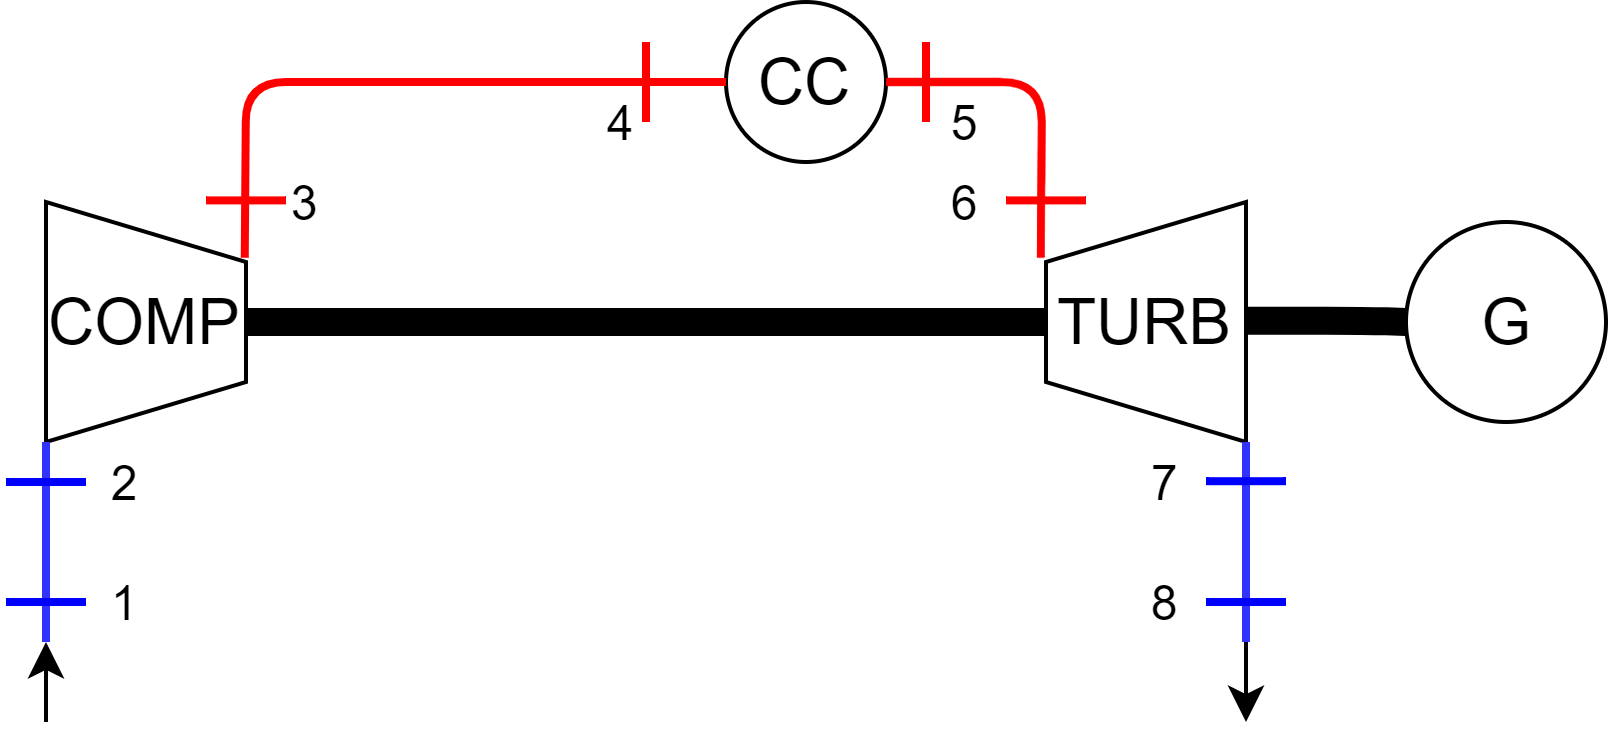
\includegraphics[width=0.6\textwidth] {GT}
\caption{Gas turbine(GT)}
\label{fig:C5_BraytonGT}
\end{figure}

The compressor and the turbine are both installed on the same shaft. Since there aren't any gearbox, the rotational speed of both component are the same. The generator (G) is also attached to the shaft to convert the generated mechanical power into electricity. 
When the machine starts, the generator becomes a motor to provide the required energy to help the turbine. Indeed, at low rotational speed the power consumed by the compressor is usually greater than the power produced by the turbine alone. 



As it is illustrated in the Figure \ref{fig:C5_BraytonGT}, the cycle can be decomposed into 8 thermodynamic states. For each connection between two elements, there are piping that will induce some pressure drops. For each of these states the temperature and pressure are measure in order to fully characterized the state. The Table \ref{tab:C5_thermo_state_GT} includes the different states emphasized on Figure \ref{fig:C5_BraytonGT}.
\begin{longtable}[c]{@{}lcc@{}}
\caption{Thermodynamic states - gas cycle (GT)}
\label{tab:C5_thermo_state_GT}\\
\toprule
\textbf{State n\degree} & $\mathbf{T}$      & $\mathbf{p}$      \\* \midrule
\endfirsthead
%
\endhead
%
\bottomrule
\endfoot
%
\endlastfoot
%
\textbf{0}              & $T_0$ = $T_{ref}$ & $p_0$ = $p_{ref}$ \\
\textbf{1}              & $T_1$ = $T_{amb}$ & $p_1$ = $p_{amb}$ \\
\textbf{2}              & $T^0_2=T_1$       & $p^0_2\leq p_1$   \\
\textbf{3}              & $T^0_3>T^0_2$     & $p^0_3>p^0_2$     \\
\textbf{4}              & $T_4=T^0_3$       & $p_4\leq p^0_3$   \\
\textbf{5}              & $T_5>>T_4$        & $p_5\leq p_4$     \\
\textbf{6}              & $T^0_6=T_5$       & $p^0_6\leq p_5$   \\
\textbf{7}              & $T^0_7<T^0_6$     & $p^0_7<p^0_6$     \\
\textbf{8}              & $T_8=T^0_7$       & $p_8=p_1<p^0_7$   \\* \bottomrule
\end{longtable} 
Where the state \textbf{0} corresponds to the reference conditions. It is worth to note that for the compressor and the turbine, the stagnation quantities are used. The reason is that in this work, method to compute the Mach number haven't been considered. This is the reason why the pressure ratios and the isentropic efficiencies that will be considered for the compressor and the turbine are based on total quantities.

For each of the mentioned states, 5 thermodynamic properties are evaluated. Namely the temperature, pressure, enthalpy, entropy and density. For the last variable, the ideal gas equation (\ref{eq:C2_GP}) from the chapter \ref{C2} is used. 

A graphical representation of these states can be performed by drawing some thermodynamic diagrams. Here, the T-s and p-v diagrams have been drawn in the Figures \ref{fig:C5_Ts_GT} and \ref{fig:C5_pv_GT} respectively.

\begin{figure}[H]
     \centering
     \begin{subfigure}[b]{0.4\textwidth}
         \centering
         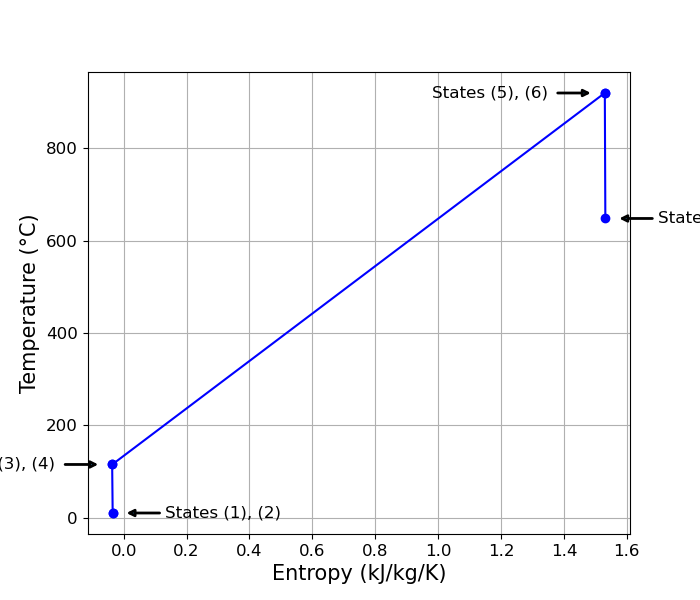
\includegraphics[width=\textwidth]{Ts_GT}
         \caption{T-s diagram - gas turbine}
         \label{fig:C5_Ts_GT}
     \end{subfigure}
     \begin{subfigure}[b]{0.4\textwidth}
         \centering
         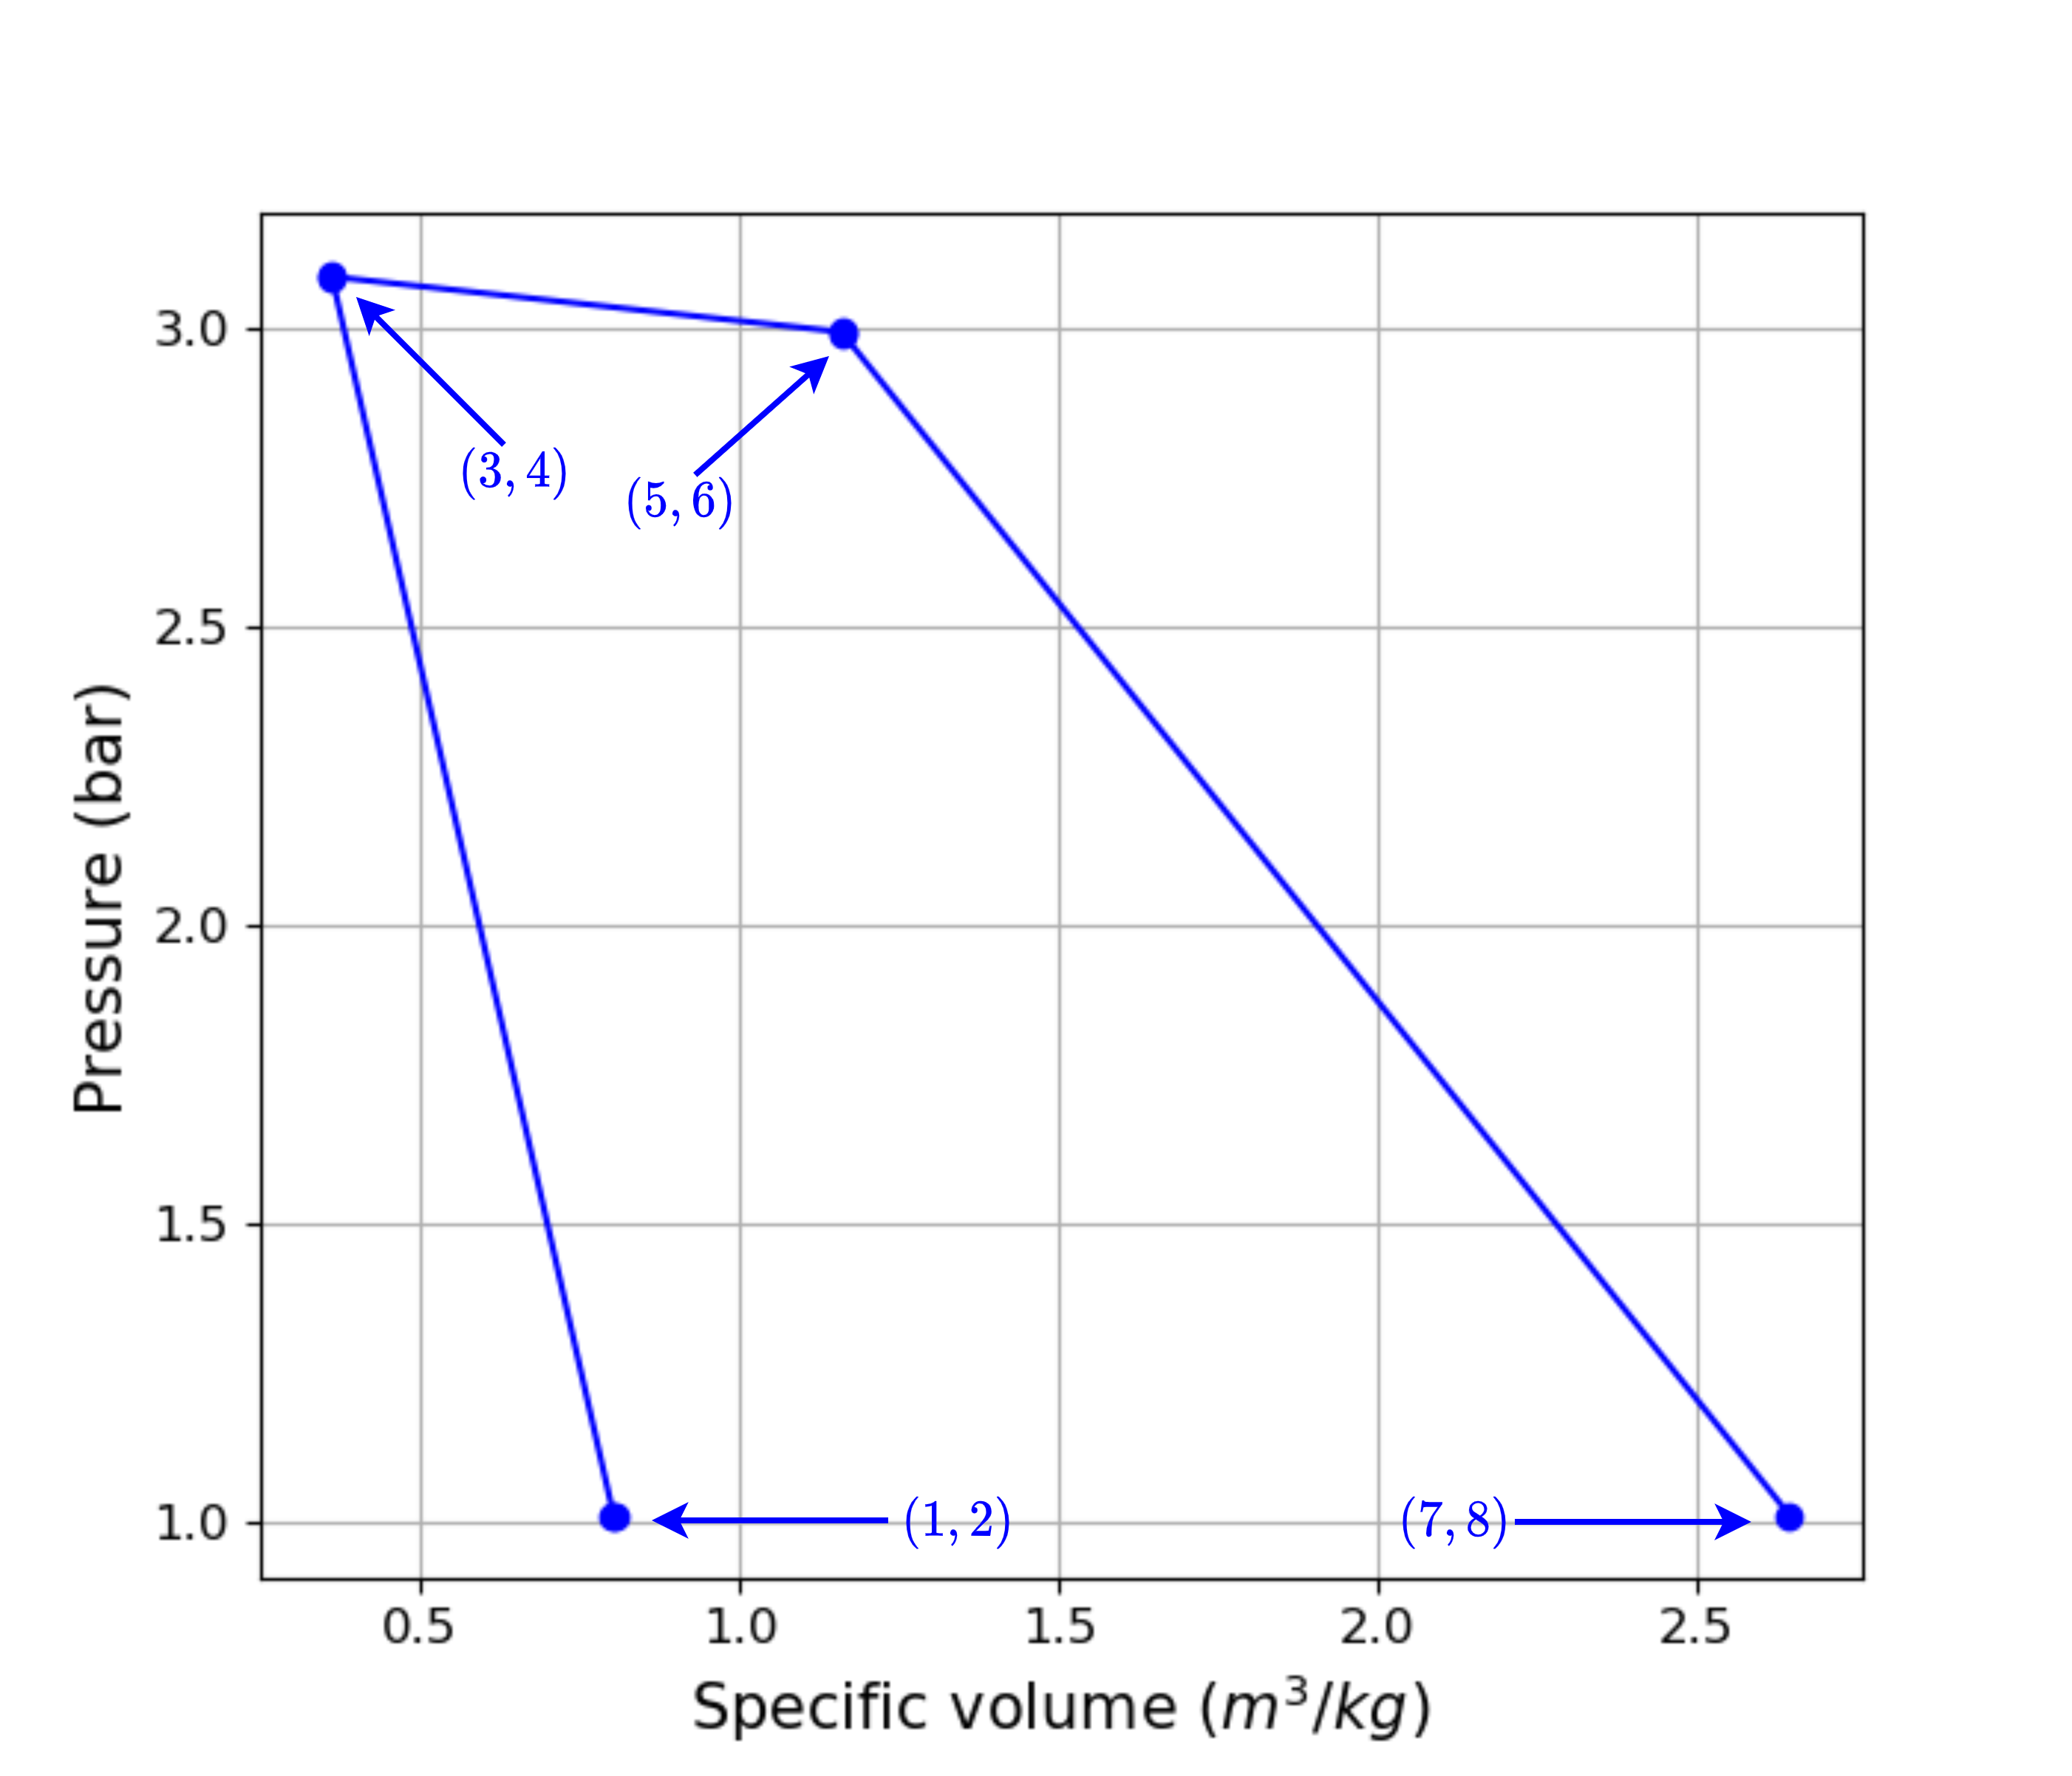
\includegraphics[width=\textwidth]{pv_GT}
         \caption{p-v diagram - gas turbine}
         \label{fig:C5_pv_GT}
     \end{subfigure}
        \caption{Thermodynamic diagrams of a gas turbine}
        \label{fig:C5_thermo_diagram_GT}
\end{figure}

These twp diagrams have been obtained considering ideal components. An ideal components is characterized by an efficiency of 100\%. This means that the there aren't any pressure drops, the isentropic efficiency $\eta_{is}$ of the compressor and the turbine is equal to 100\%, and the combustion chamber efficiency $\eta_{cc}$ is also equal to 100\%.

The p-v diagram gives an indication of the net work produced by the GT cycle. Indeed, it has been seen that the work is given by the integral (\ref{eq:C5_W}).

\begin{equation}
    \setstretch{1}
    W_{net} = \oint_{cycle}pdv\label{eq:C5_W}
\end{equation}
where $p$ is the pressure and $v$ the specific volume of the fluid.

The first diagram shows the effect of the isentropic efficiency regarding to the evolution of the entropy during the compression and the expansion. Here, since the isentropic efficiency have been set to 100\%, the entropy at the beginning and the end of the these transformations are equal.

Also, it can be noticed that at the exhaust of the cycle, the energy available within the gas is still non negligeable. A possible way of improvement will be given in the following section.

The thermal efficiency of the cycle can be computed based on the knowledge of the different states \textbf{1} to \textbf{8}. By definition, the thermal efficiency $\eta_{th}$ corresponds to the ratio (\ref{eq:C5_etath}) between the net power output $\dot{W}_{net}$ and the heat transfer rate from coming from the injected fuel.

\begin{equation}
    \setstretch{1}
    \eta_{th} = \frac{\dot{W}_{net}}{\dot{m}_{fuel}\cdot HCV_{fuel}} \label{eq:C5_etath}
\end{equation}
Where $HCV_{fuel}$ is the low heat calorific value (J/kg) of the fuel.

Based on this definition, the efficiency of the gas turbine cycle is $\eta_{th,GT} =24.58$\%. This efficiency is obtained for an ideal cycle composed of ideal components. Therefore, this represents a upper bound for any real GT cycle playing with the same level of temperature and pressure.

\section{Regenerative gas turbine (RGT)}
%%%%%%%%%%%%%%%%%%%%%%%%%%%%%%%%%%%
%%%%%                         %%%%%
%%%%%    <<regenerative>>     %%%%% 
%%%%%     <<Gas turbine>>     %%%%%
%%%%%                         %%%%%
%%%%%%%%%%%%%%%%%%%%%%%%%%%%%%%%%%%
\quad\, As seen in the previous section, the gas cycle does not have a really high efficiency. However, this efficiency can be nearly tripled by adding a regenerator to the cycle. The purpose of this heat-exchanger is to transfer part of the thermal energy from the hot gas exiting the turbine to the cold flow exiting the compressor. A schematic of the regenerative gas turbine (RGT) and the associated Ts and hp diagrams are given on Figures \ref{fig:C5_RGT} and \ref{fig:C5_thermo_diagram_RGT}. 

\begin{figure}[h]
\centering
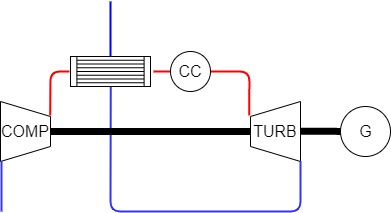
\includegraphics[width=0.5\textwidth]{RGT}
\caption{Regenerative gas turbine(RGT)}
\label{fig:C5_RGT}
\end{figure}
\begin{figure}[h]
     \centering
     \begin{subfigure}[b]{0.4\textwidth}
         \centering
         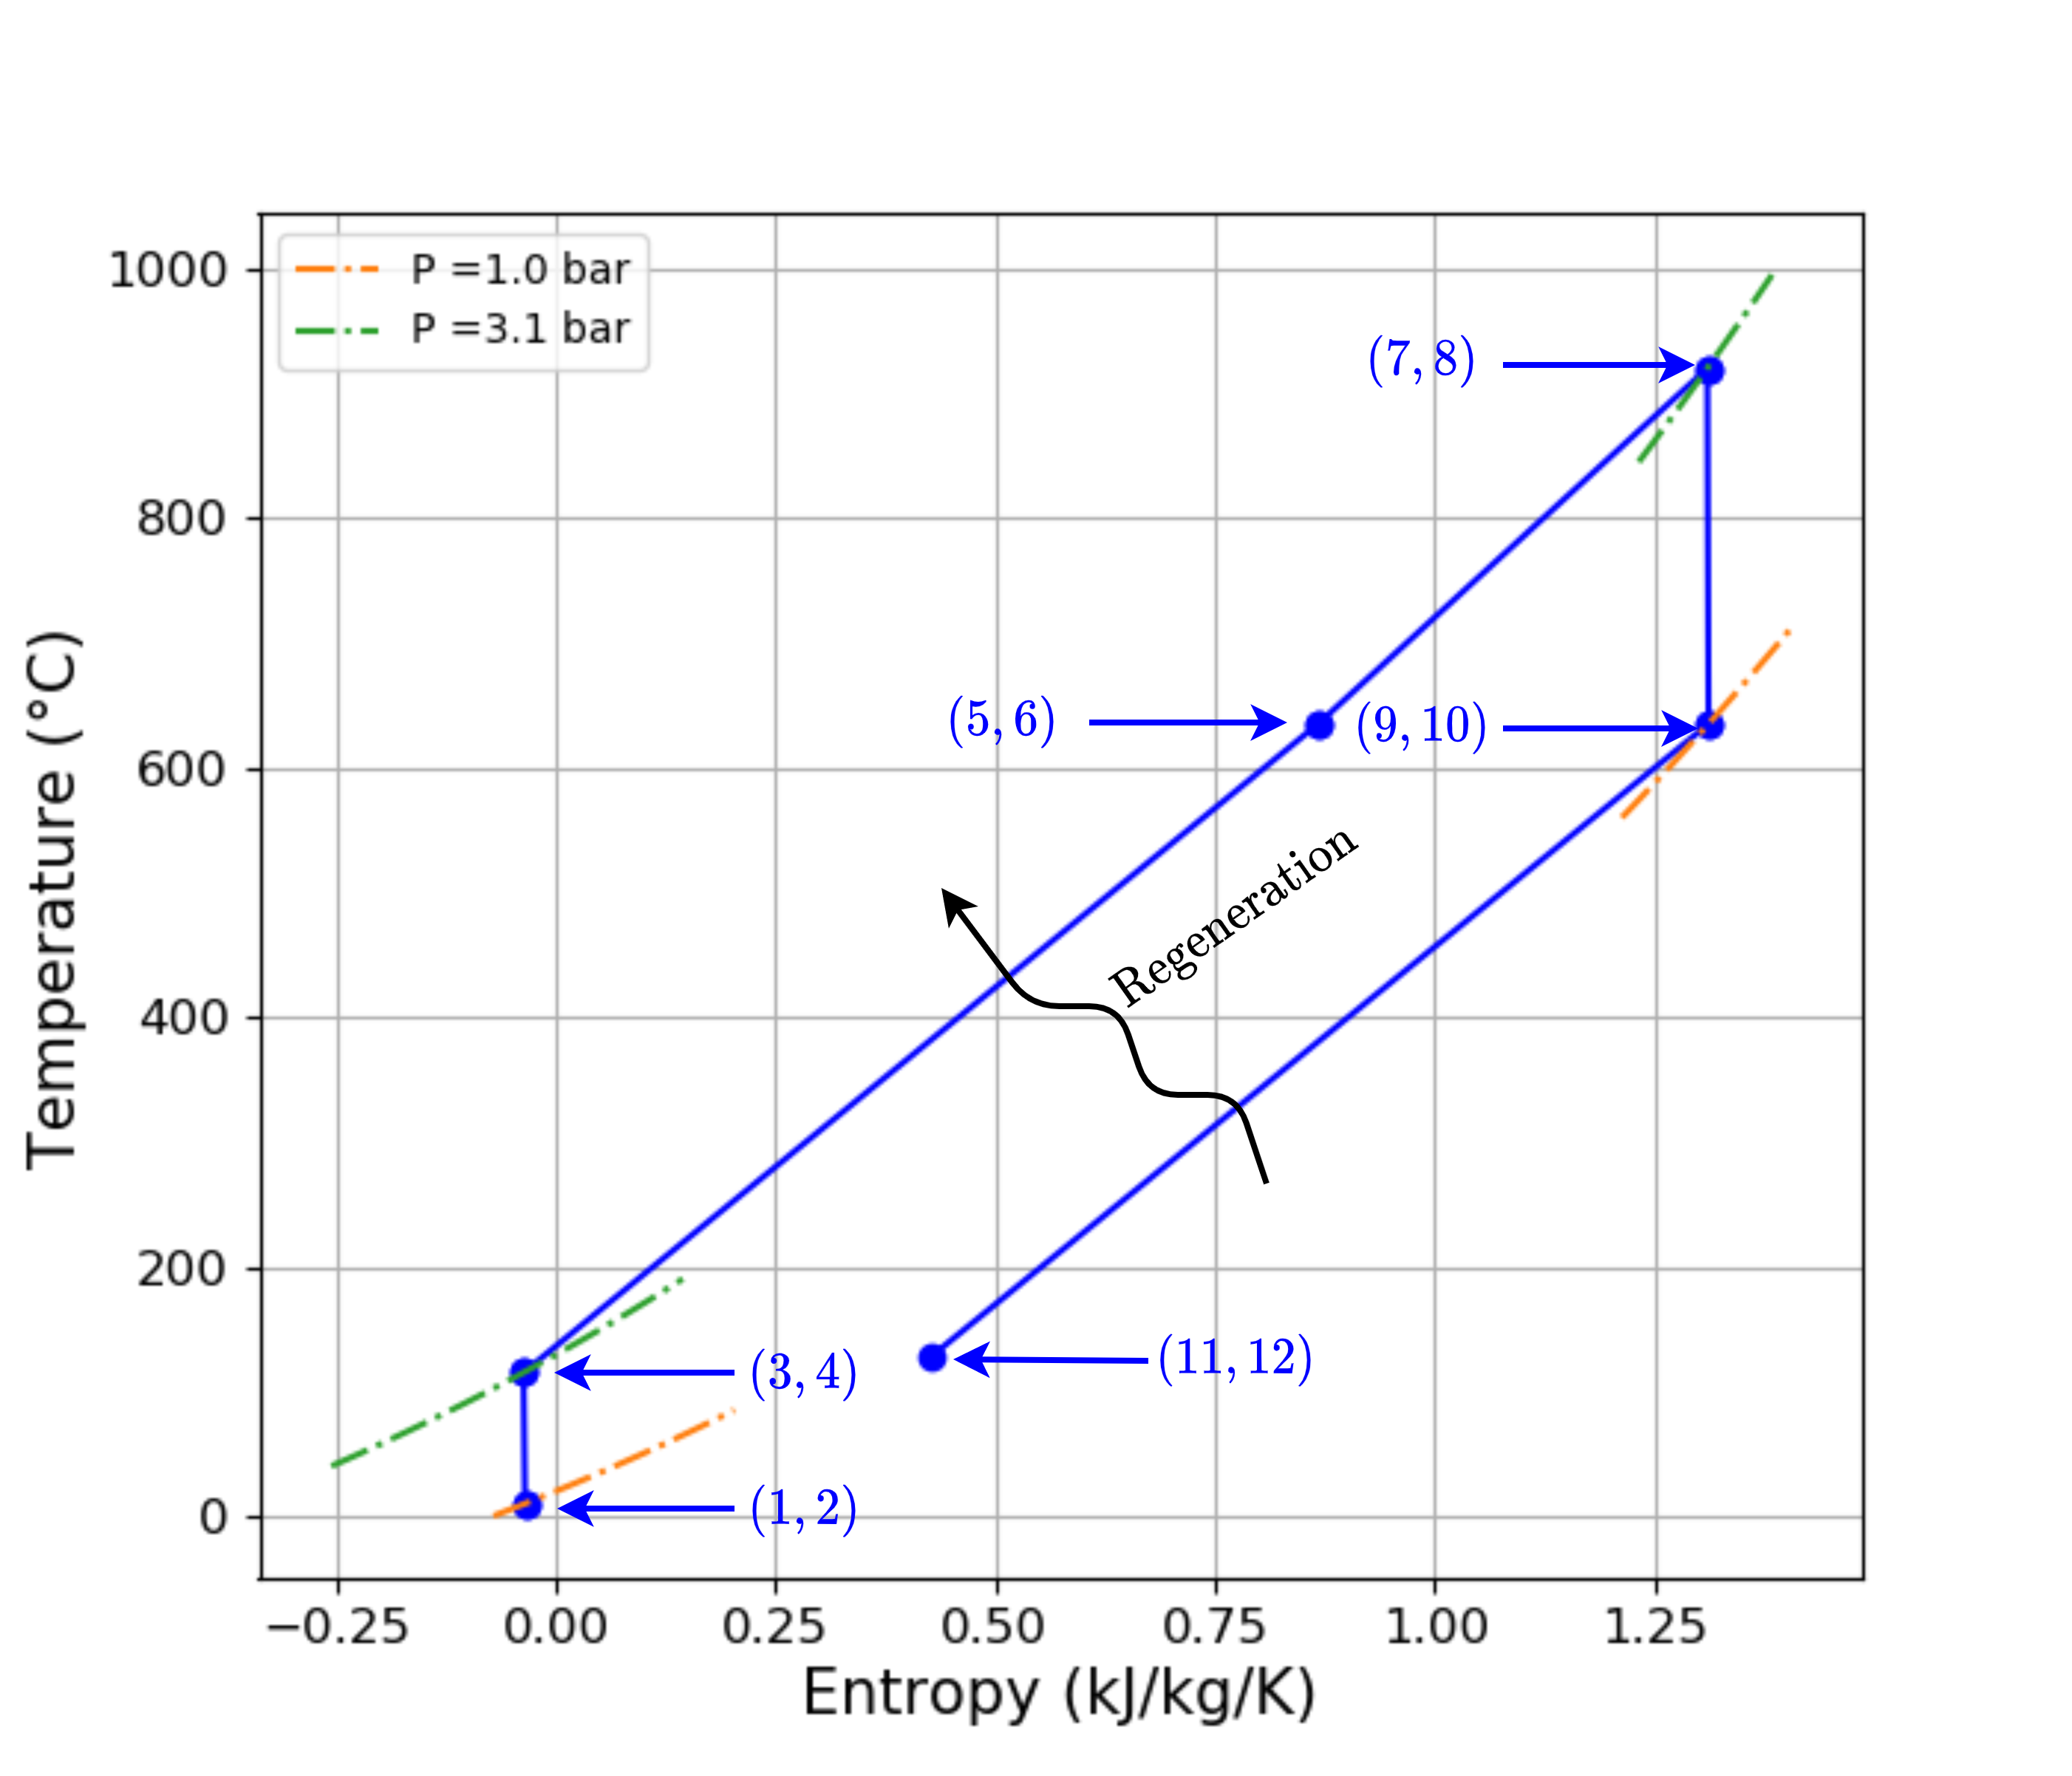
\includegraphics[width=\textwidth]{Ts_RGT}
         \caption{Ts diagram - regenerative gas turbine}
         \label{fig:C5_Ts_RGT}
     \end{subfigure}
     \begin{subfigure}[b]{0.4\textwidth}
         \centering
         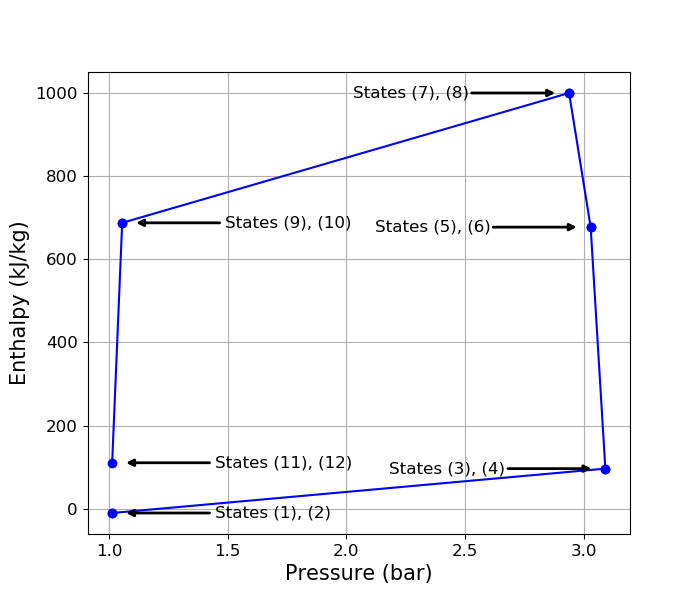
\includegraphics[width=\textwidth]{hp_RGT}
         \caption{hp diagram - regenerative gas turbine}
         \label{fig:C5_hp_RGT}
     \end{subfigure}
        \caption{Thermodynamic diagrams of a regenerative gas turbine}
        \label{fig:C5_thermo_diagram_RGT}
\end{figure}
\newpage
This has two advantages. The first one is to reduce the temperature of the gas at the exit of the cycle. The second is to reduce the fuel consumption of the system. Indeed, for an identical combustor outlet temperature (here, 950\degree C), the amount of energy that the combustion chamber has to provide to the air is lower than for the GT since the inlet temperature of the air is higher. Considering a mass flow rate of air of 180g/s, the fuel consumption goes from 3.41g/s to 1.18g/s for the RGT.

After computation, the thermal efficiency of the RGT is evaluated at $\sim$ 63\%, which is more than twice the efficiency of the GT.

Aside the regerator, a water heat exchanger (WHX) can be used to absorb the remaining from the exhaust gas to utilize it for water heating. Considering the fact that components does not have an efficiency of 100\%, the temperature at the outlet of the regenerator (state \textbf{11}) is around 200\degree C. This temperature is enough to heat up water to a target temperature of 70-80\degree C.

Even if it is beyond the scope of this master thesis, the integration of an organic rankine cycle (ORC) in place of the WHX to convert the remaining heat into electricity can also be considered\citep{Quoilin2008}.

\section{Brayton cycle - variants}
%%%%%%%%%%%%%%%%%%%%%%%%%%%%%%%%%%%
%%%%%                         %%%%%
%%%%%      <<Variants>>       %%%%%
%%%%%                         %%%%%
%%%%%%%%%%%%%%%%%%%%%%%%%%%%%%%%%%%
The GT and RGT are not the only configurations of the Brayton cycle. There exists many other involving multiple compressors, turbines, combustion chamber,etc... These configurations are illustrated in the annex \ref{annex:Brayton_variant}.

It exists many variants many variants of the Brayton cycle because engineers wanted to cover a large numbers of applications. For instance, when a large compression ratio is desired, using only one compressor is not possible. Therefore, it is necessary to split the compression between a low pressure and a high compressor. 
